% \usepackage{fontawesome5}
\usetikzlibrary{positioning,fit,arrows}


\tikzset{
    %Define standard arrow tip
    >=latex,
    %Define style for boxes
    punkt/.style={
           rectangle,
           rounded corners,
           draw=black, very thick,
           text width=7.5em,
           minimum height=2em,
           text centered},
    % Define arrow style
    pil/.style={
           ->,
           thick,}
}

\begin{adjustbox}{max height=0.95\textheight, keepaspectratio}
    \begin{tikzpicture}[node distance=3em, auto,]
     %nodes
        \node (center) {};
        \node[punkt, above=of center] (agent) {Agent \faIcon{robot}};
        % \node at (0,3.7) {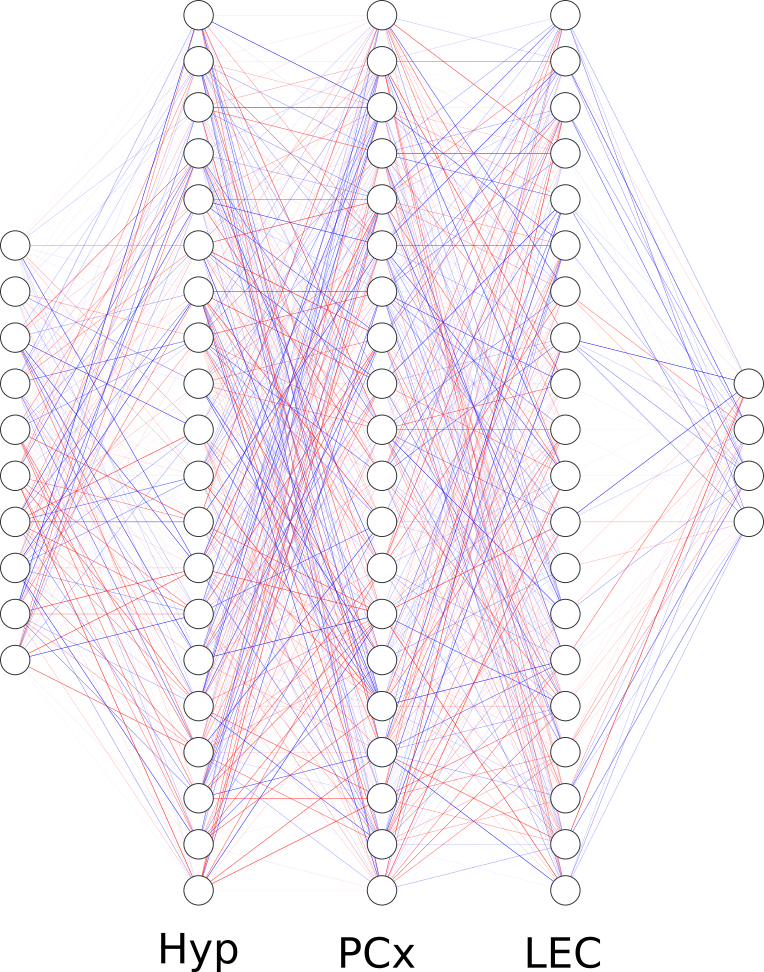
\includegraphics[height=6em]{./img/nn.svg.png}};
        \node [above=-0.2em of agent] {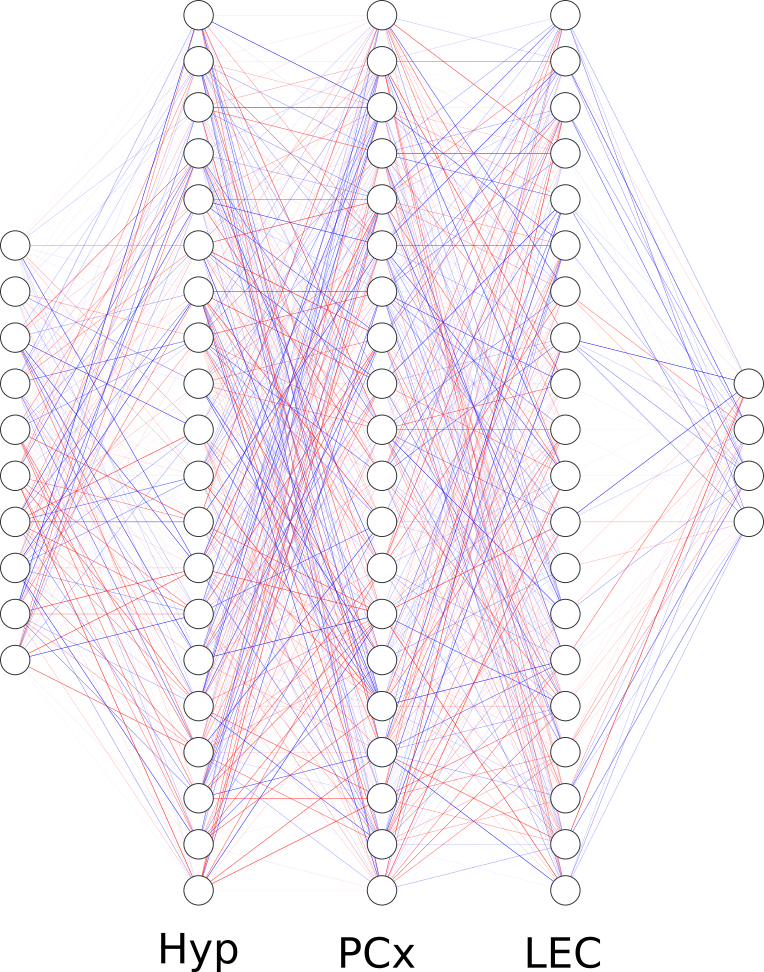
\includegraphics[height=8em]{./img/nn.svg.png}};
        \node[punkt,below=of center] (environment) {Environment \faIcon{globe}};
        \node[right=8em of center, align=center] (action) {Action\\$a_t$};
        \node[left=8em of center, align=center] (state_reward) {State, Reward\\$s_t$, $r_t$};
        \node [below=-0.2em of environment] {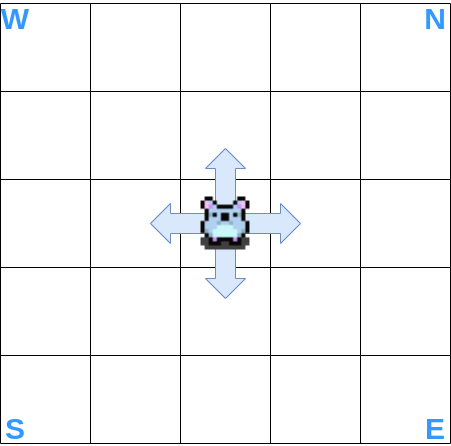
\includegraphics[height=8em]{./img/RL_environment-Allo.drawio.png}};

        \path[pil]
        (state_reward.east) edge [->, bend left=45] node {} (agent.west)
        (environment.west) edge [- , bend left=45] node {} (state_reward.east)
        (action.west) edge [->, bend left=45] node {} (environment.east)
        (agent.east) edge [-, bend left=45] node {} (action.west);
    \end{tikzpicture}
\end{adjustbox}
